\documentclass[a4paper,14pt]{extarticle}

\usepackage[utf8x]{inputenc}
\usepackage[T1,T2A]{fontenc}
\usepackage[russian]{babel}
\usepackage{hyperref}
\usepackage{indentfirst}
\usepackage{here}
\usepackage{array}
\usepackage{graphicx}
\usepackage{caption}
\usepackage{subcaption}
\usepackage{chngcntr}
\usepackage{amsmath}
\usepackage{amssymb}
\usepackage{pgfplots}
\usepackage{pgfplotstable}
\usepackage[left=2cm,right=2cm,top=2cm,bottom=2cm,bindingoffset=0cm]{geometry}
\usepackage{multicol}

\renewcommand{\le}{\ensuremath{\leqslant}}
\renewcommand{\leq}{\ensuremath{\leqslant}}
\renewcommand{\ge}{\ensuremath{\geqslant}}
\renewcommand{\geq}{\ensuremath{\geqslant}}
\renewcommand{\epsilon}{\ensuremath{\varepsilon}}
\renewcommand{\phi}{\ensuremath{\varphi}}

\counterwithin{figure}{section}
\counterwithin{equation}{section}
\counterwithin{table}{section}
\newcommand{\sign}[1][5cm]{\makebox[#1]{\hrulefill}} % Поля подписи и даты
\graphicspath{{pics/}} % Путь до папки с картинками
\captionsetup{justification=centering,margin=1cm}
\def\arraystretch{1.3}

\begin{document}

\begin{titlepage}
\begin{center}
	\textbf{Санкт-Петербургский Политехнический Университет \\Петра Великого}\\[0.3cm]
	\small Институт компьютерных наук и технологий \\[0.3cm]
	\small Кафедра компьютерных систем и программных технологий\\[4cm]
	
	\textbf{ОТЧЕТ}\\ \textbf{о лабораторной работе}\\[0.5cm]
	\textbf{<<Исследование частотных характеристик пассивных RC-цепей>>}\\[0.1cm]
	\textbf{Электротехника и Электроника}\\[10.5cm]
\end{center}

\begin{flushright}
	\begin{minipage}{0.60\textwidth}
		\begin{flushleft}
			\small \textbf{Работу выполнили студенты}\\[3mm]
			\small группа 23501/4 \hspace*{17mm} Дьячков В.В.\\[3mm]
			\small группа 23501/4 \hspace*{17mm} Ламтев А.Ю.\\[5mm]
			
			\small \textbf{Преподаватель}\\[5mm]
		 	\small \sign[3.5cm] \hspace*{8mm} к.т.н., доц. Кочетков Ю.Д.\\[0.5cm]
		\end{flushleft}
	\end{minipage}
\end{flushright}

\vfill

\begin{center}
	\small Санкт-Петербург\\
	\small \the\year
\end{center}
\end{titlepage}

\section{Цель работы}

Целью данной работы являются ознакомление с принципом действия электронных стабилизаторов напряжения, их настройка и исследование, расчети силовых звеньев.

\section{Чертеж схемы исследуемого устройства}

\begin{figure}[H]
\begin{center}
	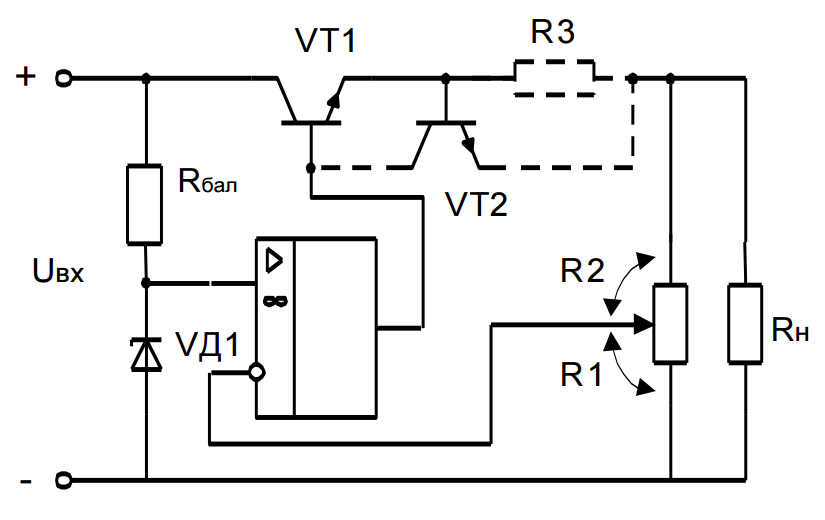
\includegraphics[scale=0.55]{scheme}
	\caption{Компенсационный стабилизатор}
\end{center}
\end{figure}

\vspace{-0.5cm}

\section{Исходные данные}

\begin{table}[H]
\begin{center}
	\caption{Исходные данные}
	\def\tabcolsep{36pt}
	\begin{tabular}{|c|c|}
		\hline 
		$\Delta U_\text{вх}$ & 20 \% \\ 
		\hline 
		$U_\text{вых}$ & 6 В \\ 
		\hline 
		$I_\text{вых}$ & 80 мА \\  
		\hline 
		$U_\text{кэ\ min}$ & 2.5 В \\ 
		\hline 
	\end{tabular} 
\end{center}
\end{table}

\newpage

\section{Теоретические расчеты и зависимости}

\begin{displaymath}
	U_\text{вых\ пульс} = 0.1 \cdot ( U_{\text{вых}\ макс} + U_{\text{кэ}\ мин} ) = 0.1 \cdot ( 6.6 + 2.5 ) = 0.91 \text{ В}
\end{displaymath}

\begin{displaymath}
\begin{aligned}
	U_{\text{вх}\ min} &= U_{\text{вых}\ max} + U_{\text{кэ}\ min} + 0.5 \cdot U_{\text{вых}\ пульс} = \\ &= 6.6 + 2.5 + 0.5 \cdot 0.91 = 9.6 \text{ В}
\end{aligned}
\end{displaymath}

\begin{displaymath}
\begin{aligned}
	U_\text{вх\ max} &= U_\text{вх\ min} + 2 \cdot \Delta U_\text{вх\ пульс} + 0.5 \cdot U_\text{вх\ пульс} = \\ &= 9.6 + 2 \cdot 0.2 \cdot 9.6 + 0.5 \cdot 0.91 = 13.9 \text{ В}
\end{aligned}
\end{displaymath}

\begin{displaymath}
	U_\text{вх\ ном} = \frac{U_{min} + U_{max}}{2} = \frac{9.6 + 13.9}{2} = 11.75 \text{ В}
\end{displaymath}

\begin{displaymath}
	R_\text{б} = \frac{U_\text{вх} - U_\text{ст}}{I_\text{ст}} = \frac{11.75 - 3}{5 \cdot 10^{-3}} = 1750 \text{ Ом}
\end{displaymath}

\paragraph{TODO} Как считать пределы изменения $I_\text{н}$ -- вопрос. Но мы почему-то меняем от 40 до 400 мА.

\begin{displaymath}
	R_\text{н} = \frac{U_\text{вых ном}}{0.5 \cdot I_{\text{вых}\ max}} = \frac{6}{0.5 \cdot 0.4} = 30 \text{ Ом}
\end{displaymath}

\section{Экспериментально снятые зависимости}

\subsection{Зависимость $U_\text{вых}$ от $U_\text{вх}$}

В таблице \ref{tab:u_in} и на рисунке \ref{fig:u_in} приведена зависимость $U_\text{вых}$ от $U_\text{вх}$.

\begin{table}[H]
\begin{center}
	\caption{Зависимость $U_\text{вых}$ от $U_\text{вх}$}
	\label{tab:u_in}
	\def\tabcolsep{40pt}
	\pgfplotstabletypeset[col sep=comma,
	    columns={u_in,u_out},
	    column type/.add={|c|}{},
	    columns/u_in/.style={fixed, precision=2, zerofill, column name={$U_\text{вх}$, В}},
	    columns/u_out/.style={fixed, precision=2, zerofill, column name={$U_\text{вых}$, В}},
	    every nth row={1}{before row=\hline},
	    every head row/.style={before row=\hline, after row=\hline},
	    every last row/.style={after row=\hline}
	   ]{data/u_in.csv}
\end{center}
\end{table}

\begin{figure}[H]
\begin{center}
	\begin{tikzpicture} [every plot/.append style={thick}]
		\begin{axis}[
			height=0.4\textheight,
			width=0.9\textwidth,
			xlabel={$U_\text{вх}$, В},
			ylabel={$U_\text{вых}$, В},
			xlabel near ticks,
			ylabel near ticks,
			axis x line = middle,
			axis y line = left,
			xmin=0,
			xmax=32,
			ymin=0,
			ymax=7,
%			xtick={0,4,...,28},
			grid=major
		]
		\addplot table[x=u_in,y=u_out,col sep=comma]{data/u_in.csv};
		\end{axis}
	\end{tikzpicture}
	\caption{Зависимость $U_\text{вых}$ от $U_\text{вх}$}
	\label{fig:u_in}
\end{center}

\end{figure}

Из рис. \ref{tab:u_in} видно, что заданное напряжение на выходе $U_\text{вых} = 6$ В было достигнуто при $U_\text{вх} \approx 12$ В.

\subsection{Зависимость $U_\text{вых}$ от $I_\text{н}$}

В таблице \ref{tab:i_n} и на рисунке \ref{fig:i_n} приведена зависимость $U_\text{вых}$ от $I_\text{н}$. 

\begin{table}[H]
\begin{center}
	\caption{Зависимость $U_\text{вых}$ от $I_\text{н}$}
	\label{tab:i_n}
	\def\tabcolsep{45pt}
	\pgfplotstabletypeset[col sep=comma,
	    columns={i_n,u_out},
	    column type/.add={|c|}{},
	    columns/i_n/.style={fixed, column name={$I_\text{н}$, мА}},
	    columns/u_out/.style={fixed, precision=2, zerofill, column name={$U_\text{вых}$, В}},
	    every nth row={1}{before row=\hline},
	    every head row/.style={before row=\hline, after row=\hline},
	    every last row/.style={after row=\hline}
	   ]{data/i_n.csv}
\end{center}
\end{table}

\begin{figure}[H]
\begin{center}
	\begin{tikzpicture} [every plot/.append style={thick}]
		\begin{axis}[
			height=0.2\textheight,
			width=0.9\textwidth,
			xlabel={$I_\text{н}$, мА},
			ylabel={$U_\text{вых}$, В},
			xlabel near ticks,
			ylabel near ticks,
			axis x line = middle,
			axis y line = left,
			xmin=0,
			xmax=450,
			ymin=5.6,
			ymax=6.4,
			grid=major
		]
		\addplot table[x=i_n,y=u_out,col sep=comma]{data/i_n.csv};
		\end{axis}
	\end{tikzpicture}
	\caption{Зависимость $U_\text{вых}$ от $I_\text{н}$}
	\label{fig:i_n}
\end{center}
\end{figure}

Из рисунка \ref{fig:i_n} видно, что выходное напряжение $U_\text{вых} \approx const = 6$ В при изменении $I_\text{н}$ в заданном пределе, следовательно оно не зависит от него.

\subsection{Зависимость $U_\text{вых}$ от $U_\text{вх}$}

В таблице \ref{tab:u_in_2} и на рисунке \ref{fig:u_in_2} приведена зависимость $U_\text{вых}$ от $U_\text{вх}$ при переносе $R_\text{бал}$ на выход стабилизатора.

\begin{table}[H]
\begin{center}
	\caption{Зависимость $U_\text{вых}$ от $U_\text{вх}$}
	\label{tab:u_in_2}
	\def\tabcolsep{40pt}
	\pgfplotstabletypeset[col sep=comma,
	    columns={u_in,u_out},
	    column type/.add={|c|}{},
	    columns/u_in/.style={fixed, precision=2, zerofill, column name={$U_\text{вх}$, В}},
	    columns/u_out/.style={fixed, precision=2, zerofill, column name={$U_\text{вых}$, В}},
	    every nth row={1}{before row=\hline},
	    every head row/.style={before row=\hline, after row=\hline},
	    every last row/.style={after row=\hline}
	   ]{data/u_in_2.csv}
\end{center}
\end{table}

\begin{figure}[H]
\begin{center}
	\begin{tikzpicture} [every plot/.append style={thick}]
		\begin{axis}[
			height=0.4\textheight,
			width=0.9\textwidth,
			xlabel={$U_\text{вх}$, В},
			ylabel={$U_\text{вых}$, В},
			xlabel near ticks,
			ylabel near ticks,
			axis x line = middle,
			axis y line = left,
			xmin=0,
			xmax=32,
			ymin=0,
			ymax=7,
%			xtick={0,4,...,28},
			grid=major
		]
		\addplot table[x=u_in,y=u_out,col sep=comma]{data/u_in_2.csv};
		\end{axis}
	\end{tikzpicture}
	\caption{Зависимость $U_\text{вых}$ от $U_\text{вх}$}
	\label{fig:u_in_2}
\end{center}
\end{figure}

Из рис. \ref{tab:u_in_2} видно, что заданное напряжение на выходе $U_\text{вых} = 6$ В было достигнуто при $U_\text{вх} \approx 9$ В. Таким образом, в данной схеме заданное выходное напряжение было достигнуто при меньшем входном напряжении.

\section{Анализ экспериментальных вычислений}

\section{Выводы}

Значение $K_\text{ст}$, вычисленное в ходе эксперимента, близко к уточненному теоретическому значению ($\delta = 6.6~\%$). Таким образом, теоретические формулы \ref{eq:k_st} и \ref{eq:r_out}  являются верными.

\end{document}